\documentclass[letterpaper]{article}
\title{
  UKF estimate of IMU-Camera Calibration\\
  \Large{16-831 Final Project: Fall 2011}
}
\author{Andrew Chambers, Natasha Kholgade, and Marynel V\'azquez}
\date{}
\usepackage[margin=1in]{geometry}
\usepackage{amsmath}
\usepackage{amssymb}
\usepackage{url}
\usepackage{graphicx}
\usepackage{color}
\usepackage{subfigure}
\usepackage{hyperref}
\newcommand{\bb}[1]{\mathbf{#1}}

\begin{document}

\maketitle

\section{Introduction}

In this project, we estimate the calibration (relative rotation and translation) between a rigidly connected camera and IMU using an unscented Kalman filter. Calibrating a camera-IMU setup is the first step in sensor fusion research. Our filter and motion simulator are the first steps in creating an open-source calibration toolbox for sensor fusion enthusiasts. 

The state vector in our unscented Kalman filter (UKF) consists of the camera-to-IMU rotation and translation, as well as the orientation and position of the IMU in the world coordinate system, the velocity in world space, the gravity vector, and the biases of the IMU's accelerometer and the gyroscope. The IMU-camera setup moves in the world space, and the camera images a set of world points with known locations in the world space. The imaged points form the measurement in our system. We predict the next state of the system from the current state by propagating a set of sigma points and noisy inertial measurements through the process model. We correct the state whenever a measurement is obtained from the camera. We synthesize the data used in this project, and we report results from the unscented Kalman filter on the noisy synthesized data.

\section{Related Work}
\label{sec:related_work}

Previous approaches to determine the relative position and rotation or calibration between a camera and IMU have been labor intensive, required special equipment, or limited to calibration for the rotation only. These previous approaches include measuring by hand, using estimated values from a CAD program during mechincal design, or surveying techniques where the physical housing of the IMU and camera are measured by a laser scanner \cite{Johnson_fieldtesting}.  More interesting calibration strategies have estimated calibration using data directly from the IMU and camera themselves. Lobo and Dias provide a rotation-only calibration toolbox called InerVis Matlab Toolbox \cite{Lobo:2009:Online}, which requires aligning a checkboard target with gravity and comparing the IMU's measurement of gravity. In later work, Lobo and Dias develop methods for the calibration of translation using specialized equipment such as a turntable  \cite{lobo2007relative}. Unfortunately this approach requires the user to rotate the whole IMU and camera system around the IMU's center. Practically this can be very difficult for systems mounted on vehicles. More recent work has determined the relative rotation and translation as part of a filtering framework using only a standard checkboard pattern.  Mirzaei and Roumeliotis \cite{mirzaei2008kalman} estimate the relative calibration parameters as one of their state variables in an extended Kalman filter. They iterate the correction step because of the high nonlinearity of the observation model. Kelly and Sukhatme \cite{2011:kelly:article} address the high nonlinearity of the visual observation by proposing the use of an unscented Kalman filter.

\section{UKF Formulation}
\label{sec:UKF}

In general, we follow the unscented Kalman filter formulation by Kelly
and Sukhatme \cite{2011:kelly:article}. This section 
summarizes important aspects of the filtering process and some
implementation details.

\subsection{System State}
In our system, we will ultimately estimate the world space position
and orientation of the IMU, $\bb{p}_I^W(t)$ and
${\overline{q}}_I^W(t)$, the velocity of the IMU-camera setup in world
space, $\bb{v}^W$, the biases for the gyroscope and accelerometer,
$\bb{b}_g(t)$ and $\bb{b}_a(t)$, the gravity vector, $\bb{g}^W(t)$,
and, of course, the position and orientation of the camera with
respect to the IMU, $\bb{p}_C^I$ and $\overline{q}_C^I$ (i.e. the
translation and rotation between the devices). The latter two are the
calibration parameters we intend to estimate, and they do not change
over time. The state vector, $\bb{x}_s(t)$ has $26 \times 1$
variables.
\begin{equation}
\bb{x}_t=\begin{bmatrix} (\bb{p}_I^W(t))^T & ({\overline{q}}_I^W(t))^T  & (\bb{v}^W(t))^T  & (\bb{b}_g(t))^T &  (\bb{b}_a(t))^T & (\bb{g}^W(t))^T  & (\bb{p}_C^I)^T & (\overline{q}_C^I)^T\end{bmatrix}
\label{eq:UKF-state}
\end{equation}

The process model uses IMU measurements as control inputs along the same
vein as Kelly and Sukhatme \cite{2011:kelly:article}. We model the accelerometer and
gyroscope biases as Gaussian random walk processes driven by zero mean
noise $\bb{n}_{aw}$ and $\bb{n}_{gw}$, with covariances $\bb{Q}_{aw}$
and $\bb{Q}_{gw}$, and we model their additive noise by zero mean
noise $\bb{n}_g$ and $\bb{n}_a$, with covariances $\bb{Q}_a$ and
$\bb{Q}_g$. The differential equations describing the state evolution
are:
\begin{align}
\dot{\bb{p}}_I^W &=\bb{v}^W \\ 
\dot{\overline{q}}_I^W&=\frac{1}{2}\begin{bmatrix}0 & -(\omega^I)^T \\ \omega^I & -[ \omega^I ]_{\times} \end{bmatrix} \overline{q}_I^W \nonumber\\
\dot{\bb{v}}^W &=\bb{a}^W  \nonumber\\
\dot{\bb{g}}^W &=\bb{0}_{3 \times 1}  \nonumber\\
\dot{\bb{b}}_g&=\bb{n}_{gw}  \nonumber\\
\dot{\bb{b}}_a&=\bb{n}_{aw}  \nonumber\\
\dot{\bb{p}}_C^I&=\bb{0}_{3 \times 1} \nonumber\\
\dot{\overline{q}}_C^I&=\bb{0}_{4 \times 1} \nonumber
\end{align}
The measured acceleration and gravity are given as
\begin{align}
\omega_m&=\omega^I+\bb{b}_g+\bb{n}_g  \\
\bb{a}_m&=\bb{C}^T(\overline{q}_I^W)(\bb{a}^W-\bb{g}^W)+\bb{b}_a+\bb{n}_a \nonumber
\end{align}
The entire process noise mean and covariance are
\begin{align}
\bb{n}=\begin{bmatrix} \bb{n}_{gw} \\ \bb{n}_{aw} \\ \bb{n}_g\\ \bb{n}_a \end{bmatrix}, \bb{Q}=\begin{bmatrix} \bb{Q}_{gw} & & & \\ & \bb{Q}_{aw} & & \\ & & \bb{Q}_g & \\ & & & \bb{Q}_a \end{bmatrix}
\end{align}

During measurement, the camera images the world points,
$\bb{p}_{l_i}^W$ (which in our current system, we assume are
known). To take the world points from the world coordinate system to
the camera's coordinate system $\bb{p}_{l_i}^C$, we apply the rotation
and orientation of the IMU in the world coordinate system, and those
of the camera with respect to the IMU:
\begin{align}
\bb{p}_{l_i}^C=(\bb{C}(\overline{q}_C^I))^T \left((\bb{C}(\overline{q}_I^W))^T \left(\bb{p}_{l_i}^W-\bb{p}_I^W\right) -\bb{p}_C^I \right)
\end{align}
We model the projected points $u_i$ and $v_i$ in the camera's coordinate system with additive measurement noise. 
\begin{align}
\bb{z}_i=\begin{bmatrix} u_i \\ v_i \end{bmatrix}&=\begin{bmatrix} x_i' \\ y_i' \end{bmatrix}+\eta_i \\
\begin{bmatrix} x_i' \\ y_i' \\ 1 \end{bmatrix} & \equiv K\begin{bmatrix} x_i \\ y_i  \\ z_i \end{bmatrix} \nonumber
\end{align}
The noise $\eta$ is modeled as zero mean with a covariance matrix $\bb{R}$.

\subsection{Unscented Kalman Filter equations}

In the unscented Kalman filter, at every time step, a set of sigma
points is estimated by jittering the state at that time step
strategically along significant directions of the augmented covariance
matrix. These significant directions correspond to eigenvectors of the
augmented covariance matrix. The \emph{a priori} predicted state is a
weighted average of the sigma points. When a measurement comes in, the
sigma points are fed to the measurement model to get an estimate of
the measurement, and the estimate of the state and the covariance
matrix is corrected by computing a Kalman gain matrix.

The augmented state and covariance updated from the time instant
$t_{k-1}$ is generated by tacking on the noise mean and covariance to
the original state and covariance matrix:
\begin{align}
\bb{\hat{x}}_a^+(t_{k-1})=\begin{bmatrix}\bb{\hat{x}}^+(t_{k-1}) \\ \bb{0}_{12 \times 1}\end{bmatrix}, \bb{P}_a^+(t_{k-1})=\begin{bmatrix} \bb{P}^+(t_{k-1}) & \\  & \bb{Q} \end{bmatrix}
\end{align}
The $N$ sigma points consist of the augmented state at $t_{k-1}$ and
the state jittered positively and negatively along the columns of the
matrix $\bb{S}$ found by the Cholesky decomposition of the augmented
covariance matrix.
\begin{align}
\bb{S} &=\sqrt{(\lambda+N) \bb{P}_a^+(t_{k-1})} \\
^0\chi_a(t_{k-1})&=\bb{\hat{x}}_a^+(t_{k-1}) \nonumber\\
^l\chi_a(t_{k-1})&=\bb{\hat{x}}_a^+(t_{k-1}) + ^l\bb{S}(t_{k-1}), l={1,...,N} \nonumber\\
^{2N+l}\chi_a(t_{k-1})&=\bb{\hat{x}}_a^+(t_{k-1})- ^l\bb{S}(t_{k-1}), l={1,...,N} \nonumber
\label{eq_sigmapoints}
\end{align}
Here $\lambda$ is a constant specified as
$\lambda=\alpha^2(N+\beta)-N$, $\alpha$ is a small number (we use
$\alpha=.1$), and $\beta=2$. Weights are computed for the sigma points
as:
\begin{align}
^0W_m&=\frac{\lambda}{\lambda+N} \\
^0W_c&=\frac{\lambda}{\lambda+N}+\left(1-\alpha^2+\beta\right) \nonumber\\
^jW_m&=^jW_c=\frac{1}{2(\lambda+N)} \nonumber
\end{align}
The sigma points are propagated through the process model, and the
\emph{a priori} estimate of the state and covariance matrix is
calculated using the propagated sigma points and the weights.
\begin{align}
^i\chi_a(t_k)&=\bb{f}(^i\chi_a(t_{k-1})), i=0,...,2N \\
\bb{\hat{x}}^-(t_k)&=\sum_{i=0}^{2N} \text{} ^iW_m \text{}^i\chi(t_k) \nonumber\\
\bb{P}^-(t_k)&=\sum_{i=0}^{2N} \text{} ^iW_c \left( ^i\chi(t_k)-\bb{\hat{x}}^-(t_k)\right) \left( ^i\chi(t_k)-\bb{\hat{x}}^-(t_k)\right)^T \nonumber
\end{align}

When measurement arrives from the camera, the sigma points are
propagated through the measurement model to get an estimate of the
measurement $\bb{\hat{z}}(t_k)$
\begin{align}
^i \gamma(t_k) &= \bb{h}(^i \chi(t_k)), i=0,...,2N \\
\bb{\hat{z}}(t_k) &=\sum_{i=0}^{2N} \text{} ^iW_m ^i\gamma(t_k) \nonumber
\end{align}
The Kalman gain matrix is computed and used to compute the \emph{a
  posteriori} state and covariance matrix.
\begin{align}
\bb{P}_{\bb{\hat{x}\hat{z}}}(t_k)&=\sum_{i=0}^{2N} \text{} ^iW_c\left( ^i \chi(t_k) - \bb{\hat{x}}^-(t_k) \right) \left( ^i \gamma(t_k)- \bb{\hat{z}}(t_k) \right)^T \\
\bb{P}_{\bb{\hat{z}\hat{z}}}(t_k)&=\sum_{i=0}^{2N} \text{} ^iW_c\left( ^i \gamma(t_k) - \bb{\hat{z}}^(t_k) \right) \left( ^i \gamma(t_k)- \bb{\hat{z}}(t_k) \right)^T \nonumber \\
\bb{K}(t_k)&=\bb{P}_{\bb{\hat{x}\hat{z}}}(t_k) \left( \bb{P}_{\bb{\hat{z}\hat{z}}}(t_k) + \bb{R} \right)^{-1} \nonumber \\
\bb{\hat{x}}^+(t_k)&=\bb{\hat{x}}^-(t_k)+\bb{K}(t_k)\left( \bb{z}(t_k)-\bb{\hat{z}}(t_k) \right) \nonumber \\
\bb{P}^+(t_k)&=\bb{P}^-(t_k)-\bb{K}(t_k)\bb{P}_{\bb{\hat{z}\hat{z}}}(t_k)(\bb{K}(t_k))^T \nonumber
\end{align}

\subsection{Representing Rotations with Quaternions}

As described in Kelly and Sukhatme \cite{2011:kelly:article}, the unscented
Kalman filter updates the state by computing the barycentric mean of
the sigma points. In general the barycentric mean of unit quaternions
$\overline{q}_I^W$ and $\overline{q}_C^I$ will not lie on the unit
sphere, and we require a different parametrization for their
update. We make use of the technique called UnScented QUaternion Estimator, 
or USQUE from \cite{crassidis2003unscented}.
This technique represents rotations in the filter state vector as full 4 element quaternions
but expresses the state covariance as a 3-by-3 matrix in modified Rodrigues parameters (MRPs). 
The state covariance represents the uncertainly expressed in MRPs around the expected rotation.
If we did not express state covariance using a 3 parameter representation, 
it would result in a rank deficient covariance matrix since there are only 3 degrees of freedom in rotation.
Similar to Euler's angles and all 3 parameter representations of rotation, MRPs exhibit singularities 
at certain rotations. MRPs are singular at $360^\circ$ but since we are using the MRPs to
express an error, this is not a problem since the error in rotation should never approach $360^\circ$.

For small errors in rotation, the modified Rodrigues parameter $\delta \bb{e}$ is given as:
\begin{align}
\delta \bb{e}=\frac{\delta \bb{q}}{1+\delta q_0},
\end{align}
where $\delta \bb{q}$ and $\delta q_0$ are each the vector and scalar
portion of the error quaternion. At time step $t_k$, we start off with
a mean error quaternion of $^0\delta
\bb{\hat{e}}_I^W(t_{k-1})=\bb{0}_{3 \times 1}$ and $^0\delta
\bb{\hat{e}}_C^I=\bb{0}_{3 \times 1}$. The MRP part of the sigma
points is computed $^j \bb{\hat{e}}_I^W(t_{k-1})$ in terms of these
mean MRPs using \ref{eq_sigmapoints}, and corresponding quaternions
are propagated as
\begin{align}
^j \hat{\overline{q}}_I^W(t_{k-1})=^j \delta \hat{\overline{q}}_I^W(t_{k-1}) \otimes \hat{\overline{q}}^{W+} (t_{k-1})
\end{align}
The sigma points are passed through the process model, and before
computing the barycentric mean, the mean quaternion is divided out to
get the error quaternion at $t_k$.
\begin{align}
^j \delta \hat{\overline{q}}_I^W(t_k)=^j \hat{\overline{q}}_I^W(t_k) \otimes \left( ^0 \hat{\overline{q}}_I^W(t_k)\right)^{-1}
\end{align}
The process of multiplying error vectors to get unit quaternions is
repeated before passing the sigma points to the measurement model, and
they are re-computed before obtaining the Kalman gain matrix. For the
IMU-camera orientation $\overline{q}_C^I$, the error quaternions are
used only when a measurement comes in.

\section{Data synthesis}
\label{Datasynth}
To test our system, we built two simulators to synthesize input data for the filter. The first simulator creates a list of translational accelerations and rotational velocities for the system. For example, a very simple list could be constant values for all accelerations and angular velocities. Another option would be to create a list of varying values based on sinesoidal waves at different frequences. The synthesized inertial data is integrated forward in time to generate the ground truth path for the IMU. At each time step, 3D points are projected into the camera for the ground truth pixel coordinates. The ground truth inertial and camera data are perturbed by Gaussian noise and a random walk bias term and used as the inputs for the Kalman filter. As we will explain next, generating a specific output trajectory such as a figure-eight is very difficult to do using only inertial inputs.

We noticed that the above method produces a camera path where the camera does not consistently look at the points. The camera image plane might intersect the landmarks in world space, in which case, the points projections would lie at infinity. The camera may unrealistically look away from the points, or it may go too far from them. We needed a method that would produce a reasonable camera path, where the camera is within reach of the landmarks, and is consistently looking at them. In our second synthesis method, we manually defined control points of a Bezier curve around the $3D$ points, and we generated a smooth camera path using the Bezier curve. This path defined the position of the camera, $\bb{p}_C^W(t)$ at different instants of time. To specify the orientation $\hat{\overline{q}}_C^W(t)$, we computed a look at vector $v_{lookat}$ from the camera position $\bb{p}_C^W$ to the mean of the landmarks, $\bb{p}_{\mu}^C$. We defined an up vector, $v_{up}$ to lie along the $z$-axis by default, and we computed a third orthogonal vector, $v_{orth}=v_{lookat} \times v_{up}$. We computed the orientation in matrix form as $\begin{bmatrix}v_{orth} &v_{up}& v_{lookat}\end{bmatrix}$, and we converted it to the quaternion $\hat{\overline{q}}_C^W(t)$. Figure \ref{synthcontrolpts} shows the control points specified for the camera path, and Figure \ref{synthpath} shows the camera path as it looks at the points, the IMU attached rigidly to the camera, and the projected points in the camera's image plane.
\begin{figure}[t]
\centering
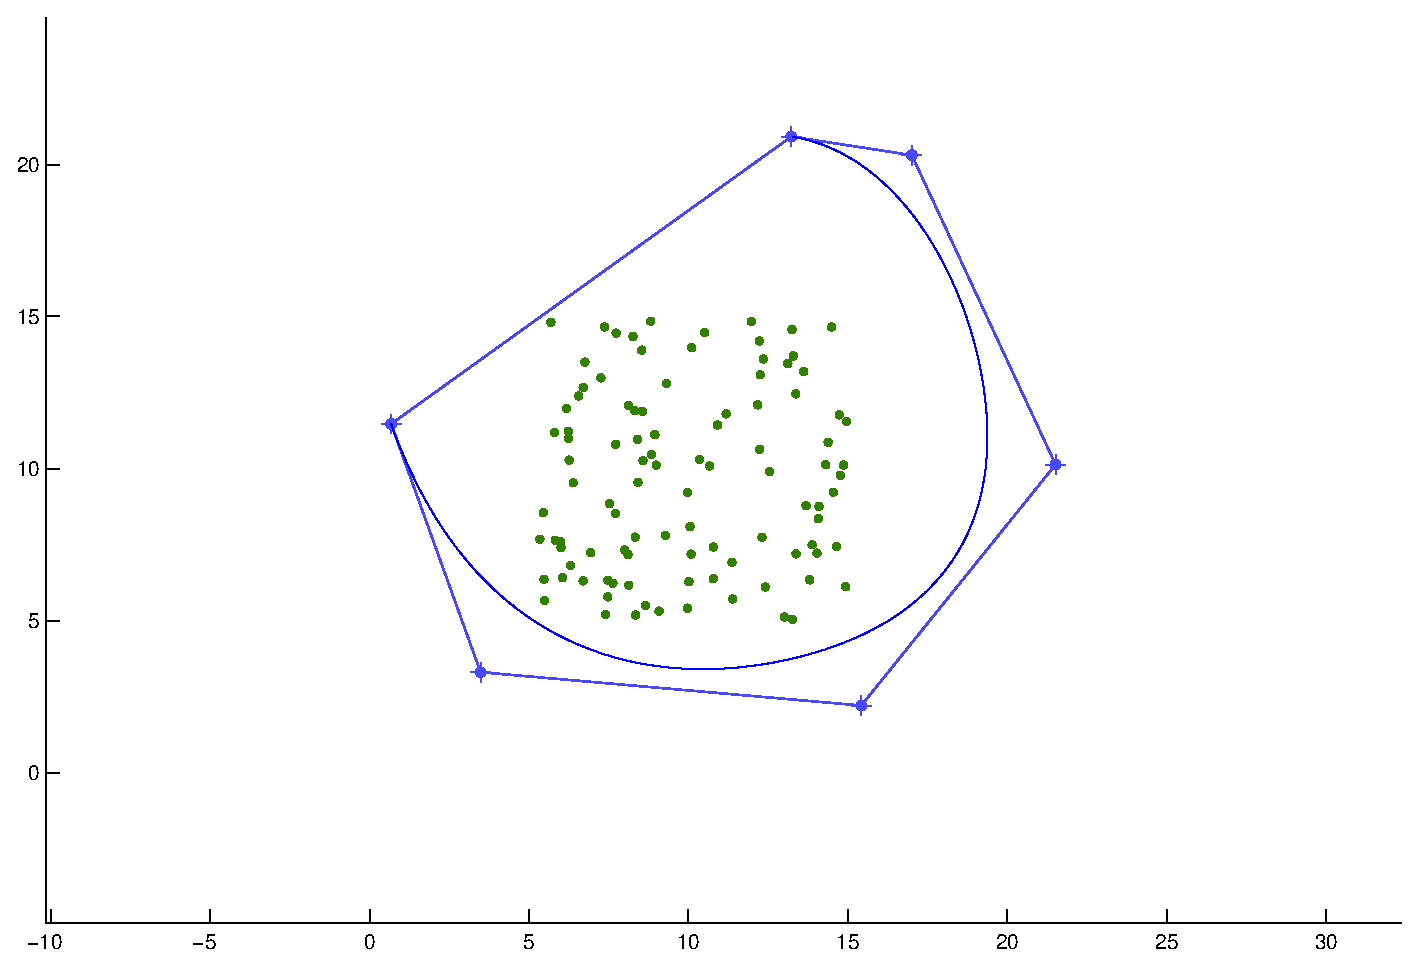
\includegraphics[width=.5\linewidth]{synth_controlpts.eps}
\caption{Top view of landmarks and control points used to generate camera path}
\label{synthcontrolpts}
\end{figure}
\begin{figure}[t]
\centering
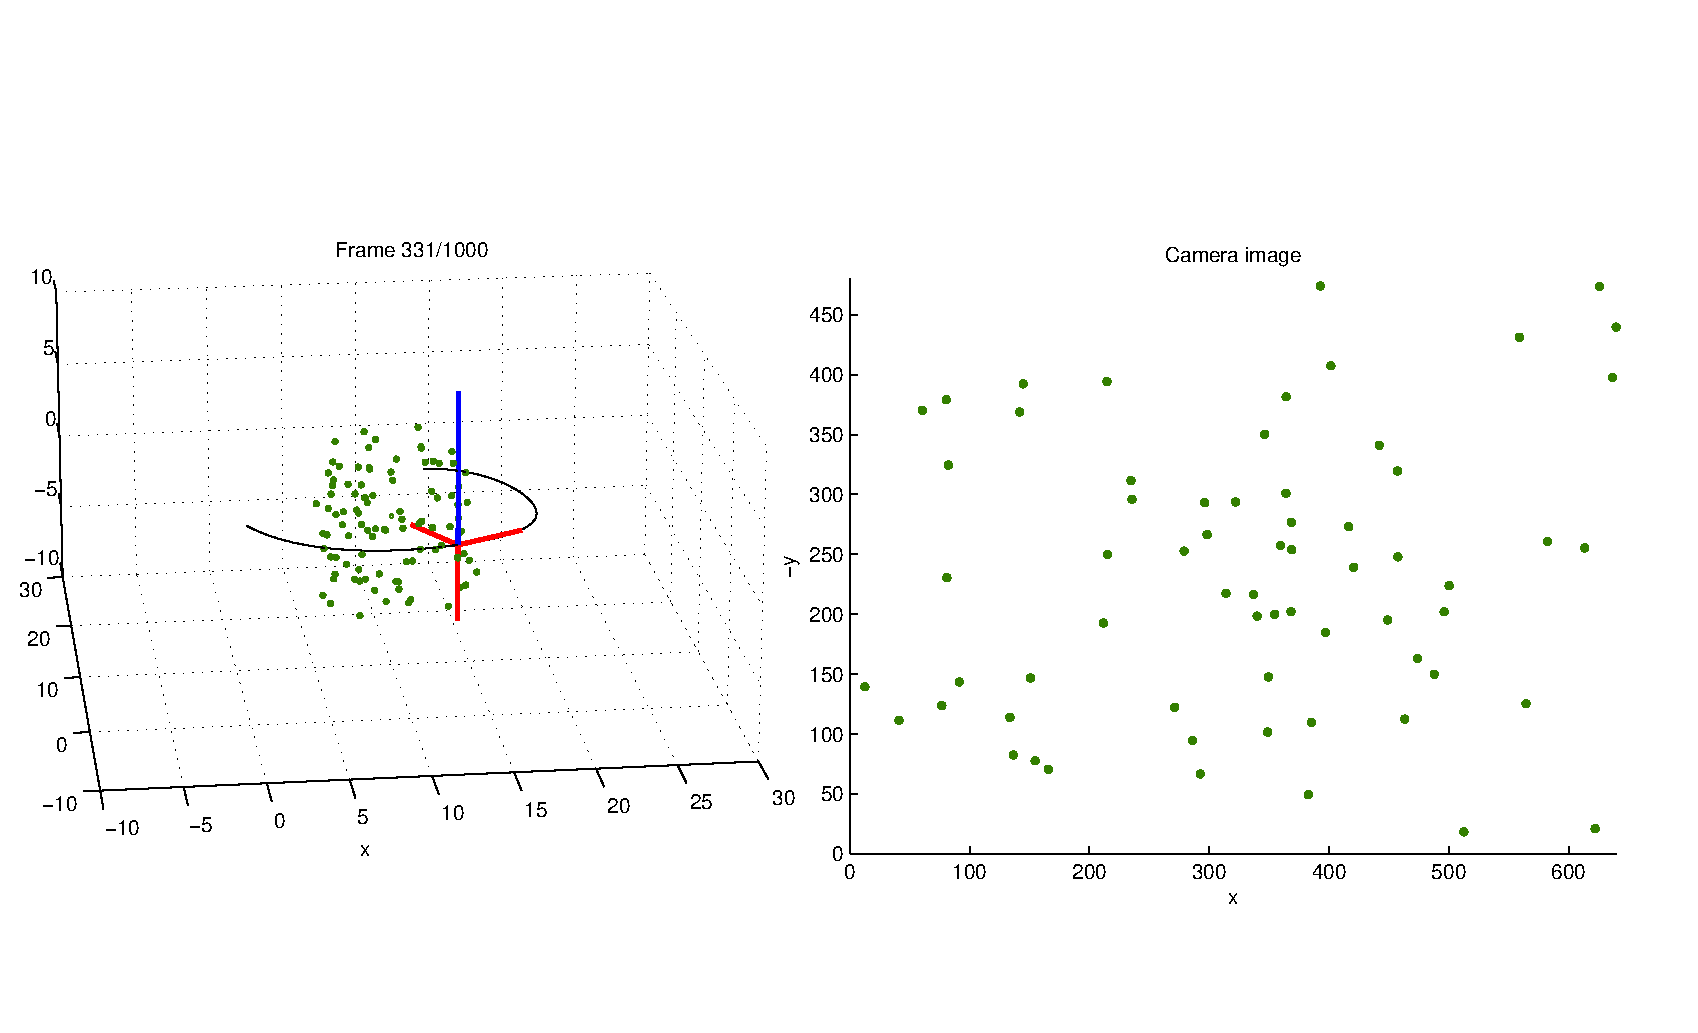
\includegraphics[width=\linewidth]{synth_path.eps}
\caption{Left: Camera path in the world space in black, landmarks in green, IMU-camera setup in blue, camera rotation matrix (look-at, up, and orthogonal vectors) in red. Right: projections of the landmarks in the image plane of the camera.}
\label{synthpath}
\end{figure}

\section{Results}

%% We decided to implement the filter progressively given the complexity
%% of the state space. We considered a reduced number of unknowns and a
%% very simple model at the beginning. The following subsections detail
%% our progress towards a complete toolbox for sensor-to-sensor
%% calibration.

%% \subsection{Estimating rigid body translation}

%% \begin{figure}[h!tbp]
%% \centering
%% 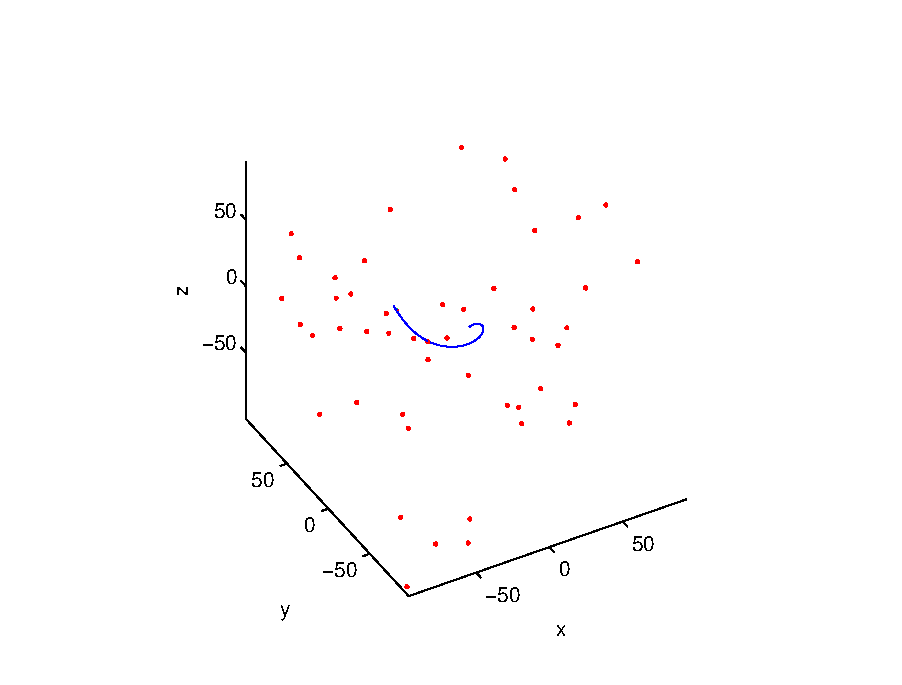
\includegraphics[width=0.5\linewidth]{uniform_points}
%% \caption{Automatically generated landmarks (red points) in our simulated
%%   world. The blue line depicts the uniform velocity path used for the
%%   rigid body translation test.}
%% \label{fig:TranslationTest-uniformPoints}
%% \end{figure}


%% Our first filter implementation consists of estimating the
%% position in 3D space of the rigid body sensor suite. We assume that we have a "world velocity sensor," which provided noisy estimates of the system's velocity in the world frame. No bias or gravity terms needed to be considered in this model.

%% We generated a ground truth path for the sensor suite using a simple motion simulator which generates motions from a vector of constant angular velocity and constant acceleration. These motions determine the grouth truth for world velocity, position, and orientation of the sensors at every point in time. We corrupt the grouth truth velocity and provide it to the filter as a sensor measurement at the correction step.
%% Our state vector has a dimensionality of $3$ in this test,
%% instead of $26$ as in (\ref{eq:UKF-state}). The process noise
%% covariance is a $3 \times 3$ diagonal matrix.
%% \begin{equation}
%% \bb{x}_t=\begin{bmatrix} p_{I_x}^W(t) & p_{I_y}^W(t) & p_{I_z}^W(t) \end{bmatrix} 
%% \hspace{4em}
%% Q = \begin{bmatrix} 
%% \sigma_x^2 & 0 & 0\\ 
%% 0 & \sigma_y^2 & 0\\ 
%% 0 & 0 & \sigma_z^2
%% \end{bmatrix} 
%% \label{eq:TranslationTest-stateVec}
%% \end{equation}

%% We automatically generate landmarks by uniformly scattering 3D points
%% in our simulated world, and projected them into our simulated camera
%% sensor. Figure \ref{fig:TranslationTest-uniformPoints} depicts a
%% possible distribution of landmarks in our simulated world. When landmarks are projected into the camera frame and measured as pixel coordinates, we add indepedant Gaussian noise to the pixel coordinates to simulate the real-world behavior of cameras.

%% \begin{figure}[h!tbp]
%% \centering
%% 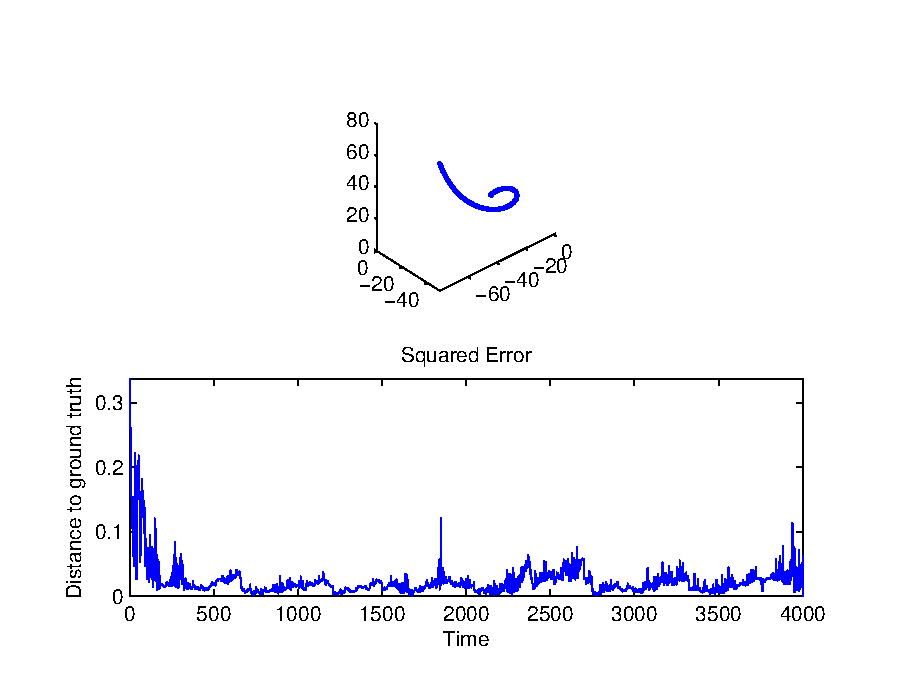
\includegraphics[width=0.85\linewidth]{estimated_position_and_error}
%% \caption{Estimated 3D world position of the camera and IMU from the UKF and squared error distance between estimated position and grouth truth}
%% \label{fig:TranslationTest-estimatedPosition}
%% \end{figure}

%% Fig. {\ref{fig:TranslationTest-estimatedPosition}} shows the 3D position estimate for the IMU in the world frame from the unscented Kalman filter. We also plot the squared distance between the ground truth and the estimated position at each step in time. There is a large initial error because we initialize the UKF with an error of 0.5 meters in each axis. Even with this large initial error, the filter is able to converge and track the true position.

% TODO. Might be a good idea to regenerate this picture with whatever
% point distribution we used before submitting the report..

We carried out various simulation studies while implementing the
UKF. We started estimating only the position of the IMU in space
($\bb{p}_I^W(t)$), and gradually incremented the complexity of the
state vector. For brevity, we only report results obtained for the
state vector presented in equation (\ref{eq:UKF-state}).

We modeled a sensor beam of $30$ cm in length, with the camera and the
IMU positioned at its extremes. We generated $10$ seconds of synthetic
motion data, as explained
in Section \ref{Datasynth} for the IMU at a sampling rate of $100$ Hz. We limited the motion to a maximum
linear acceleration of $1.23$ m/s$^2$, and maximum angular velocity of
$0.55$ rad/s (approx. $31^\circ$/s).  Then, we placed a total of 30
visual landmarks near the path of the beam with the constraint that
they should almost lie in a plane,\footnote{Though the planar
  constraint is not necessary for the UKF filter to work, we wanted to
  mimic a real target-based calibration scenario
  \cite{2011:kelly:article}.} and projected them into the camera
image.  Figure \ref{fig:groundtruth} shows the synthesized path of the
IMU, as well as the set of 3D landmarks that we used as ground truth.
\begin{figure}[h!p]
\centering
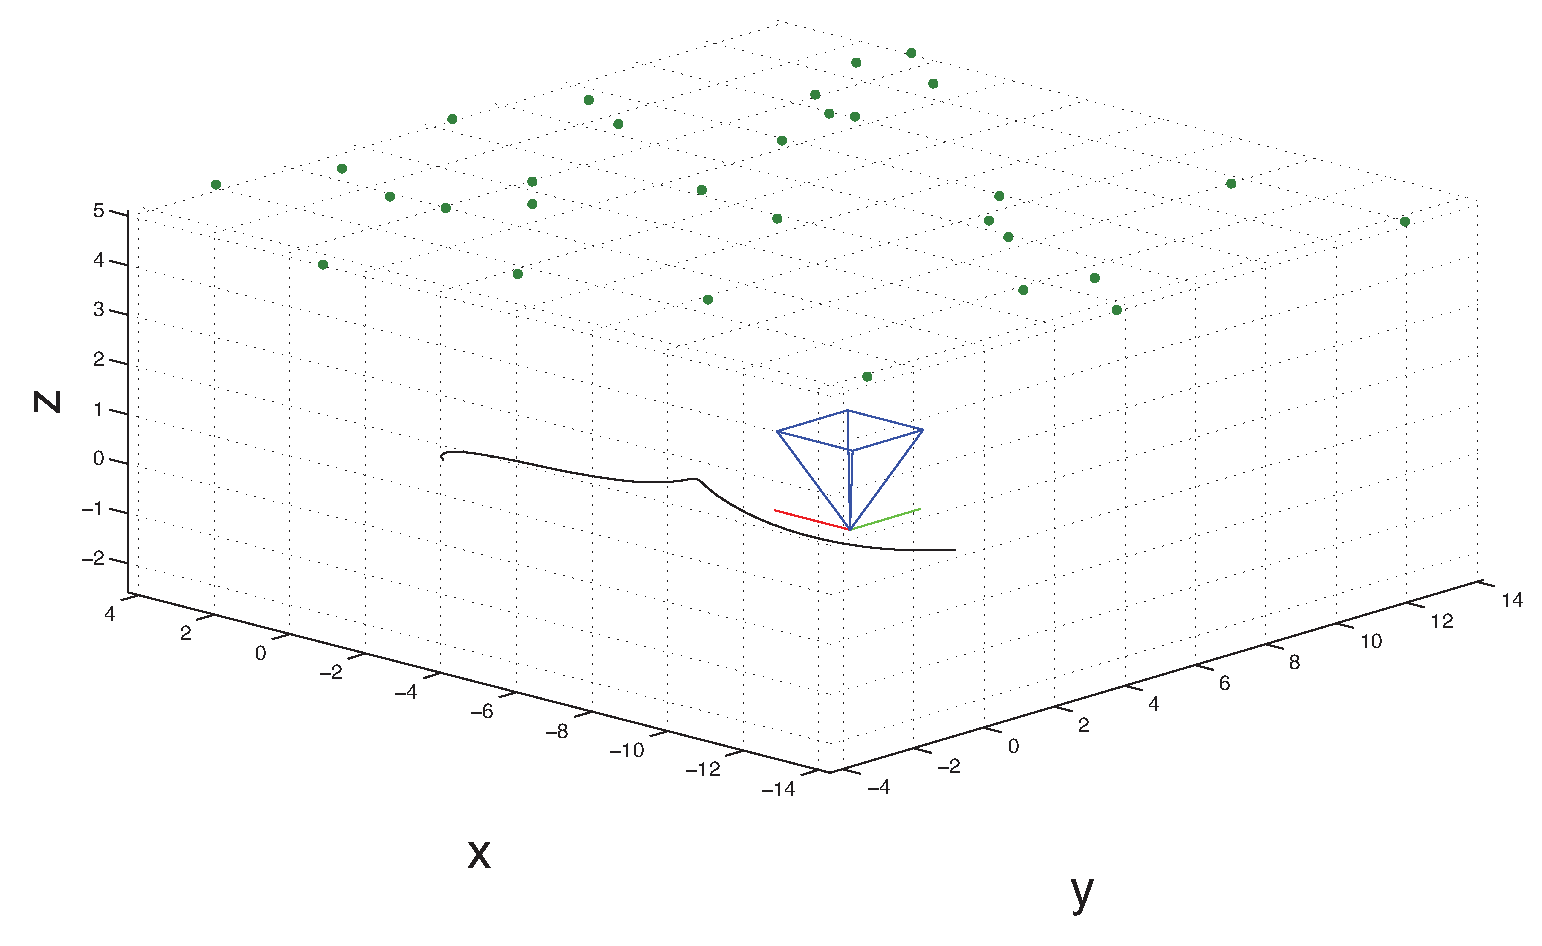
\includegraphics[width=.7\linewidth]{groundTruth.eps}
\vspace{-0.5em}
\caption{Synthesized ground truth data. The black line depicts the
  path of IMU in 3D space, while the green dots represent 3D visual
  landmarks captured by the camera (blue). The gap between the camera
  and the IMU path is due to the $30$ cm beam that keeps the sensors
  rigidly attached.}
\label{fig:groundtruth}
\end{figure}

We altered synthesized ground truth data to process measurements
similar to those obtained in the real world. The accelerations
measured by the IMU were altered with Gaussian noise of zero mean and
$0.0196$ standard deviation, plus a bias modeled as random walk (with
std $= 0.0042$). Likewise, ground truth angular velocities from the
IMU were altered with Gaussian noise of zero mean and $0.0087$
standard deviation. Gyroscope bias was also modeled as a random walk
with standard deviation of $0.0001534$.\footnote{Accelerometer and
  gyroscope noises were modeled following the specifications of the
  Microstrain\textregistered\ 3DM-GX3\textregistered\ -45 IMU.}

Some noise was also added to the 2D projections of the landmarks in
the camera image. We used zero-mean Gaussian noise with
standard deviation of $1$ in this case. Note that we assumed we were able to
distinguish between visual features, and did not tackle the problem of
wrong landmark correspondences.

\subsection{General performance}

We initialized the UKF filter with the correct initial position
$\bb{p}_I^W(0)$ of the IMU plus a random zero-mean Gaussian noise with
standard deviation of $0.8$. The initial velocity $\bb{v}^W(0)$ and
orientation $\overline{q}_I^W(0)$ of the IMU were set with their
  ground truth values plus zero-mean Gaussian noise of $0.3$ and
  $0.0349$ standard deviations, respectively. The latter corresponds
  to about $8$ degrees of deviation, computed using modified Rodrigues
  parameters (MRPs). The initial values of the relative position
  $\bb{p}_C^I$ and orientation $\overline{q}_C^I$ of the IMU and the
  camera were altered with zero-mean Gaussian noise with standard
  deviations of $1$ and $0.0218$ (approximately $5$ degrees). Finally,
  gravity $\bb{g}^W(0)$ and the biases $\bb{b}_g(0)$ and $\bb{b}_a(0)$
  were altered with Gaussian noise of zero mean and $0.1$ standard
  deviation. These values were reasonable approximations to the real
  initial state of the system.

The state covariance matrix was initialized as a diagonal matrix with
standard deviations of $0.1$, $0.0437$, $0.5$ for the position,
orientation, and velocity of the IMU. Accelerometer and gyroscope
biases were also modeled with diagonal covariance matrices with
standard deviations of $0.001$ and $0.02$, while the relative position
and orientation of the IMU and the camera were assigned $0.001$ and
$0.0306$. Gravity was the only variable with different values along
the diagonal of its state covariance matrix, having $1.7$, $1.7$, and
$0.15$ standard deviations for its x, y, and z components,
respectively. This difference accentuated the fact that estimation
errors for gravity tend to occur more along the x and y dimensions, than z.

Figure \ref{fig:generalResults} shows the average estimation error for
all state vector variables after 50 runs with the same ground truth
data. Very small errors were obtained in general.
% Check previous argument!


\begin{figure}[h!p]
\centering
\subfigure[Position error (m)]{
  \includegraphics[width=0.4\linewidth]{experiment-Distance.png}
}
\subfigure[Orientation error (degrees)]{
  \includegraphics[width=0.4\linewidth]{experiment-Orientation.png}
}
\subfigure[Velocity error (m/s)]{
  \includegraphics[width=0.4\linewidth]{experiment-Velocity.png}
}
\subfigure[Gravity error (m/s$^2$)]{
  \includegraphics[width=0.4\linewidth]{experiment-Gravity.png}
}
\subfigure[IMU-Camera distance error (m)]{
  \includegraphics[width=0.4\linewidth]{experiment-Pic.png}
}
\subfigure[IMU-Camera orientation error (deg)]{
  \includegraphics[width=0.4\linewidth]{experiment-Qic.png}
}
\subfigure[Acclerometer bias error (m/s$^2$)]{
  \includegraphics[width=0.4\linewidth]{experiment-AccelBias.png}
}
\subfigure[Gyroscope bias error (deg/s)]{
  \includegraphics[width=0.4\linewidth]{experiment-GyroBias.png}
}
\caption{Estimation error averaged across 50 runs}
\label{fig:generalResults}
\end{figure}

\subsection{Rigid body motion}

In general, the IMU should experience accelerations and rotations
along two axes for the filter to converge successfully
\cite{2011:kelly:article}. Undesired filter behaviors were observed
when this requirement was not met and, specially, when we increased
the values of the state covariance matrix that corresponded to the
relative position and orientation between the IMU and the camera. 
A typical result of the filtering process in this scenario would be
correcting for estimation errors by adjusting the distance between the
two sensors more than desired, instead of changing the current
position of the IMU in space. This would generate increasing
correlated errors for $\bb{p}_I^W(t)$ and $\bb{p}_C^I$, as none of
these variables would converge towards their real values.


\section{Discussion and future work}
%% The next step in the project will be to expand our filter to estimate
%% the full state vector. The most difficult part of this implementation
%% will be the quaternion predication and correction steps within the
%% Kalman filter. We are also developing a more complicated motion
%% simulator to simulate the motion and field of view for a realistic
%% camera-IMU system.
We have implemented an IMU-camera calibration system using an unscented Kalman filter. We estimate rotation and translation between the IMU and camera, as well as the position and orientation of the IMU in world space, the velocity of the system in the world, the gravity vector, and the biases of the accelerometer and gyroscope. As input we take in points in world space with known locations (as on a target), and measurements of linear acceleration and angular velocity from the IMU. We have tested our filter with data generated synthetically and augmented with varying amounts of noise. 

Our current synthesis either allows smooth acceleration of the IMU, or the realistic camera motion (with the camera looking at the landmarks) but not necessarily both for some types of paths. When the camera path is generated using Bezier curves, for some paths, the IMU acceleration may not be smooth. The camera may suddenly change orientation, causing a sudden jump in the IMU's path. This jump throws off our filter's estimates. Future work includes generating more diverse camera paths such that the IMU's acceleration is smooth. Future work also includes applying the filter to real data obtained from IMU-camera setups or devices such as the iPhone. 

\bibliographystyle{plain}
\bibliography{IVCalib-FinalReport}

\end{document}

